% Corresponding source for the AGPL-derived gallery PNG.
\RequirePackage{fix-cm}
\documentclass{article}
\usepackage[paperwidth=267.891mm,paperheight=98.2812mm,margin=5mm]{geometry}
\usepackage{fontspec}
\usepackage{xeCJK}
\IfFontExistsTF{PingFang SC}{\setCJKmainfont{PingFang SC}}{\IfFontExistsTF{Noto Sans CJK SC}{\setCJKmainfont{Noto Sans CJK SC}}{\IfFontExistsTF{Heiti SC}{\setCJKmainfont{Heiti SC}}{\setCJKmainfont{FandolHei-Regular}}}}
\usepackage{tikz}
\usetikzlibrary{arrows.meta,calc,positioning,fit,backgrounds,shapes.geometric}
\pagestyle{empty}
\newcommand{\CaptureTikZPositions}{}
% Edit shared fonts, component sizes, gaps, borders and arrows here.
\definecolor{ink0}{HTML}{000000}
\definecolor{ink1}{HTML}{555184}
\definecolor{ink2}{HTML}{FFFFFF}
\definecolor{ink3}{HTML}{CECCDF}
\definecolor{ink4}{HTML}{8482B5}
\newcommand{\FontA}{\fontsize{8.5625}{10.275}\selectfont\mdseries\color{ink0}}
\newcommand{\FontB}{\fontsize{7.49219}{8.99062}\selectfont\mdseries\color{ink0}}
\newcommand{\WidthA}{32.1094mm}
\newcommand{\HeightA}{32.1094mm}
\newcommand{\WidthB}{40.1953mm}
\newcommand{\HeightB}{40.1953mm}
\newcommand{\WidthC}{29.4141mm}
\newcommand{\HeightC}{29.4141mm}
\newcommand{\WidthD}{45.9961mm}
\newcommand{\HeightD}{45.9961mm}
\newcommand{\WidthE}{41.7773mm}
\newcommand{\HeightE}{41.7773mm}
\newcommand{\WidthF}{37.7344mm}
\newcommand{\HeightF}{30.2344mm}
\newcommand{\WidthG}{32.1094mm}
\newcommand{\HeightG}{24.6094mm}
\newcommand{\WidthH}{30.1172mm}
\newcommand{\HeightH}{22.6172mm}
\newcommand{\WidthI}{28.125mm}
\newcommand{\HeightI}{3.86719mm}
\newcommand{\WidthJ}{30.8203mm}
\newcommand{\HeightJ}{7.5mm}
\newcommand{\WidthK}{21.0938mm}
\newcommand{\HeightK}{7.26562mm}
\newcommand{\WidthL}{21.0938mm}
\newcommand{\HeightL}{7.26562mm}
\newcommand{\WidthM}{20.2734mm}
\newcommand{\HeightM}{7.26562mm}
\newcommand{\WidthN}{20.8594mm}
\newcommand{\HeightN}{7.03125mm}
\newcommand{\WidthO}{19.3359mm}
\newcommand{\HeightO}{7.03125mm}
\newcommand{\WidthP}{17.5781mm}
\newcommand{\HeightP}{7.03125mm}
\newcommand{\WidthQ}{23.4375mm}
\newcommand{\HeightQ}{4.45312mm}
\newcommand{\WidthR}{23.4375mm}
\newcommand{\HeightR}{4.45312mm}
\newcommand{\WidthS}{23.4375mm}
\newcommand{\HeightS}{4.45312mm}
\newcommand{\WidthT}{23.4375mm}
\newcommand{\HeightT}{4.45312mm}
\newcommand{\WidthU}{23.4375mm}
\newcommand{\HeightU}{7.61719mm}
\newcommand{\WidthV}{23.4375mm}
\newcommand{\HeightV}{7.61719mm}
\newcommand{\WidthW}{23.4375mm}
\newcommand{\HeightW}{7.61719mm}

% Local geometry: x right, y down; one macro call per semantic component.
\newcommand{\FeatureStack}[8]{%
\begin{scope}[shift={(#1.north west)},x=1mm,y=-1mm]
\pgfmathtruncatemacro{\lastface}{#4-1}
\foreach \i in {0,...,\lastface}{%
\ifodd\i\def\facecolor{#8}\else\def\facecolor{#7}\fi
\fill[\facecolor] ({\i*#5},{\i*#6}) rectangle ++(#2,#3);
}
\end{scope}}
\newcommand{\TensorSlab}[5]{%
\begin{scope}[shift={(#1.north west)},x=1mm,y=-1mm]
\fill[#5] (0,0)--(#2,0)--({#2+#4},#3)--(#4,#3)--cycle;
\end{scope}}

\tikzset{
border-fine/.style={draw=ink1,line width=0.21406250000000002pt,solid,line cap=round,line join=round},
edge-fine/.style={border-fine,-},
border-caption/.style={draw=ink0,line width=0.42812500000000003pt,solid,line cap=round,line join=round},
edge-caption/.style={border-caption,-},
border-layer-link/.style={draw=ink1,line width=0.42812500000000003pt,solid,line cap=round,line join=round},
edge-layer-link/.style={border-layer-link,-},
node-label/.style={border-fine,fill=ink2,rectangle,draw=none,fill=none,align=center,inner sep=0.01mm,outer sep=0pt,font=\FontA},
node-light/.style={border-fine,fill=ink3,rectangle,draw=none,fill=none,align=center,inner sep=0.01mm,outer sep=0pt,font=\FontA},
node-dark/.style={border-fine,fill=ink4,rectangle,draw=none,fill=none,align=center,inner sep=0.01mm,outer sep=0pt,font=\FontA},
node-compact/.style={border-fine,fill=ink2,rectangle,draw=none,fill=none,align=center,inner sep=0.01mm,outer sep=0pt,font=\FontB}
}

\begin{document}
\noindent% Editable native TikZ. Positive scene y points down.
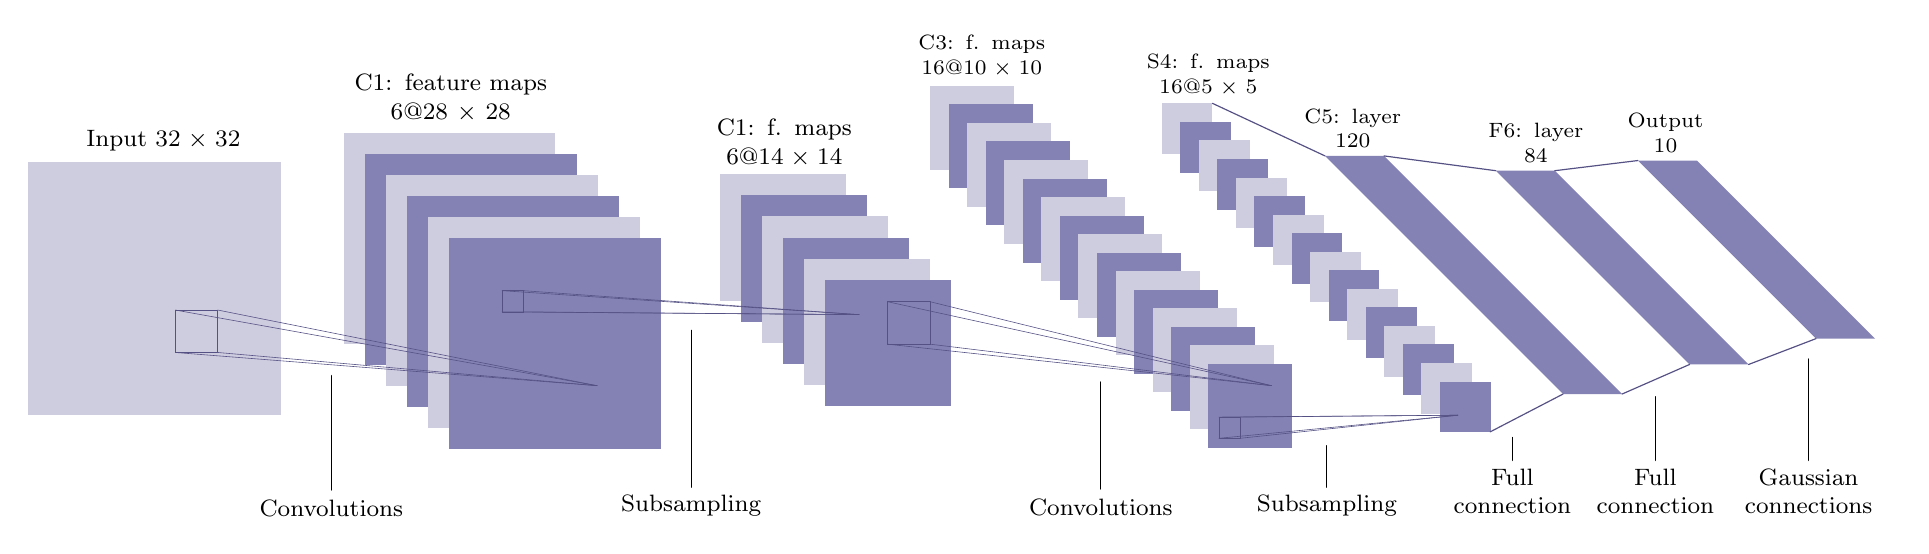
\begin{tikzpicture}[>=Latex]
\node[node-label,minimum width=\WidthA,minimum height=\HeightA,text width=\dimexpr\WidthA*1000/1000-0.02mm\relax] (input) at (18.1641mm,-32.8125mm) {};
\node[node-label,minimum width=\WidthB,minimum height=\HeightB,text width=\dimexpr\WidthB*1000/1000-0.02mm\relax] (c1) at ($(input)+(44.2383mm,-0.292969mm)$) {};
\node[node-label,minimum width=\WidthC,minimum height=\HeightC,text width=\dimexpr\WidthC*1000/1000-0.02mm\relax] (s2) at ($(c1)+(42.3047mm,0.117188mm)$) {};
\node[node-label,minimum width=\WidthD,minimum height=\HeightD,text width=\dimexpr\WidthD*1000/1000-0.02mm\relax] (c3) at ($(s2)+(35.0098mm,2.95898mm)$) {};
\node[node-label,minimum width=\WidthE,minimum height=\HeightE,text width=\dimexpr\WidthE*1000/1000-0.02mm\relax] (s4) at ($(c3)+(27.3047mm,-0.117188mm)$) {};
\node[node-label,minimum width=\WidthF,minimum height=\HeightF,text width=\dimexpr\WidthF*1000/1000-0.02mm\relax] (c5) at ($(s4)+(18.7207mm,-0.908203mm)$) {};
\node[node-label,minimum width=\WidthG,minimum height=\HeightG,text width=\dimexpr\WidthG*1000/1000-0.02mm\relax] (f6) at ($(c5)+(18.8672mm,0.9375mm)$) {};
\node[node-label,minimum width=\WidthH,minimum height=\HeightH,text width=\dimexpr\WidthH*1000/1000-0.02mm\relax] (output) at ($(f6)+(17.0508mm,2.28516mm)$) {};
\node[node-label,minimum width=\WidthI,minimum height=\HeightI,text width=\dimexpr\WidthI*1000/1000-0.02mm\relax] (input-label) at ($(input)+(1.17188mm,18.8086mm)$) {Input $32\times32$};
\node[node-label,minimum width=\WidthJ,minimum height=\HeightJ,text width=\dimexpr\WidthJ*1000/1000-0.02mm\relax] (c1-label) at ($(c1)+(-6.5625mm,24.5508mm)$) {C1: feature maps\\$6@28\times28$};
\node[node-label,minimum width=\WidthK,minimum height=\HeightK,text width=\dimexpr\WidthK*1000/1000-0.02mm\relax] (s2-label) at ($(s2)+(-6.50391mm,18.6914mm)$) {C1: f. maps\\$6@14\times14$};
\node[node-compact,minimum width=\WidthL,minimum height=\HeightL,text width=\dimexpr\WidthL*1000/1000-0.02mm\relax] (c3-label) at ($(c3)+(-16.4355mm,26.748mm)$) {C3: f. maps\\$16@10\times10$};
\node[node-compact,minimum width=\WidthM,minimum height=\HeightM,text width=\dimexpr\WidthM*1000/1000-0.02mm\relax] (s4-label) at ($(s4)+(-14.9707mm,24.5215mm)$) {S4: f. maps\\$16@5\times5$};
\node[node-compact,minimum width=\WidthN,minimum height=\HeightN,text width=\dimexpr\WidthN*1000/1000-0.02mm\relax] (c5-label) at ($(c5)+(-15.3516mm,18.6328mm)$) {C5: layer\\120};
\node[node-compact,minimum width=\WidthO,minimum height=\HeightO,text width=\dimexpr\WidthO*1000/1000-0.02mm\relax] (f6-label) at ($(f6)+(-10.957mm,15.8203mm)$) {F6: layer\\84};
\node[node-compact,minimum width=\WidthP,minimum height=\HeightP,text width=\dimexpr\WidthP*1000/1000-0.02mm\relax] (output-label) at ($(output)+(-11.543mm,14.8242mm)$) {Output\\10};
\node[node-label,minimum width=\WidthQ,minimum height=\HeightQ,text width=\dimexpr\WidthQ*1000/1000-0.02mm\relax] (op-0) at ($(c1)+(-21.7383mm,-27.5977mm)$) {Convolutions};
\node[node-label,minimum width=\WidthR,minimum height=\HeightR,text width=\dimexpr\WidthR*1000/1000-0.02mm\relax] (op-1) at ($(s2)+(-18.3398mm,-27.3633mm)$) {Subsampling};
\node[node-label,minimum width=\WidthS,minimum height=\HeightS,text width=\dimexpr\WidthS*1000/1000-0.02mm\relax] (op-2) at ($(c3)+(-1.31836mm,-30.5566mm)$) {Convolutions};
\node[node-label,minimum width=\WidthT,minimum height=\HeightT,text width=\dimexpr\WidthT*1000/1000-0.02mm\relax] (op-3) at ($(s4)+(0.0878906mm,-30.2051mm)$) {Subsampling};
\node[node-label,minimum width=\WidthU,minimum height=\HeightU,text width=\dimexpr\WidthU*1000/1000-0.02mm\relax] (op-4) at ($(c5)+(4.92188mm,-27.4805mm)$) {Full\\connection};
\node[node-label,minimum width=\WidthV,minimum height=\HeightV,text width=\dimexpr\WidthV*1000/1000-0.02mm\relax] (op-5) at ($(f6)+(4.21875mm,-28.418mm)$) {Full\\connection};
\node[node-label,minimum width=\WidthW,minimum height=\HeightW,text width=\dimexpr\WidthW*1000/1000-0.02mm\relax] (op-6) at ($(output)+(6.62109mm,-30.7031mm)$) {Gaussian\\connections};
\FeatureStack{input}{32.1094}{32.1094}{1}{0}{0}{ink3}{ink4}
\FeatureStack{c1}{26.8359}{26.8359}{6}{2.67188}{2.67188}{ink3}{ink4}
\FeatureStack{s2}{16.0547}{16.0547}{6}{2.67188}{2.67188}{ink3}{ink4}
\FeatureStack{c3}{10.6641}{10.6641}{16}{2.35547}{2.35547}{ink3}{ink4}
\FeatureStack{s4}{6.44531}{6.44531}{16}{2.35547}{2.35547}{ink3}{ink4}
\TensorSlab{c5}{7.5}{30.2344}{30.2344}{ink4}
\TensorSlab{f6}{7.5}{24.6094}{24.6094}{ink4}
\TensorSlab{output}{7.5}{22.6172}{22.6172}{ink4}
\draw[edge-caption] ($(c1.north west)+(-1.64062mm,-30.8203mm)$) -- ($(c1.north west)+(-1.64062mm,-45.3516mm)$);
\draw[edge-caption] ($(s2.north west)+(-3.63281mm,-19.8047mm)$) -- ($(s2.north west)+(-3.63281mm,-39.7266mm)$);
\draw[edge-caption] ($(c3.north west)+(21.6797mm,-37.6172mm)$) -- ($(c3.north west)+(21.6797mm,-51.2109mm)$);
\draw[edge-caption] ($(s4.north west)+(20.9766mm,-43.4766mm)$) -- ($(s4.north west)+(20.9766mm,-48.75mm)$);
\draw[edge-caption] ($(c5.north west)+(23.7891mm,-35.7422mm)$) -- ($(c5.north west)+(23.7891mm,-38.6719mm)$);
\draw[edge-caption] ($(f6.north west)+(20.2734mm,-28.7109mm)$) -- ($(f6.north west)+(20.2734mm,-36.7969mm)$);
\draw[edge-caption] ($(output.north west)+(21.6797mm,-25.1953mm)$) -- ($(output.north west)+(21.6797mm,-38.0859mm)$);
\draw[edge-fine] ($(input.north west)+(18.75mm,-18.75mm)$) -- ($(input.north west)+(24.1406mm,-18.75mm)$) -- ($(input.north west)+(24.1406mm,-24.1406mm)$) -- ($(input.north west)+(18.75mm,-24.1406mm)$) -- cycle;
\draw[edge-fine] ($(input.north west)+(18.75mm,-18.75mm)$) -- ($(c1.north west)+(32.1094mm,-32.1094mm)$);
\draw[edge-fine] ($(input.north west)+(24.1406mm,-18.75mm)$) -- ($(c1.north west)+(32.1094mm,-32.1094mm)$);
\draw[edge-fine] ($(input.north west)+(24.1406mm,-24.1406mm)$) -- ($(c1.north west)+(32.1094mm,-32.1094mm)$);
\draw[edge-fine] ($(input.north west)+(18.75mm,-24.1406mm)$) -- ($(c1.north west)+(32.1094mm,-32.1094mm)$);
\draw[edge-fine] ($(c1.north west)+(20.0391mm,-20.0391mm)$) -- ($(c1.north west)+(22.7344mm,-20.0391mm)$) -- ($(c1.north west)+(22.7344mm,-22.7344mm)$) -- ($(c1.north west)+(20.0391mm,-22.7344mm)$) -- cycle;
\draw[edge-fine] ($(c1.north west)+(20.0391mm,-20.0391mm)$) -- ($(s2.north west)+(17.6953mm,-17.8125mm)$);
\draw[edge-fine] ($(c1.north west)+(22.7344mm,-20.0391mm)$) -- ($(s2.north west)+(17.6953mm,-17.8125mm)$);
\draw[edge-fine] ($(c1.north west)+(22.7344mm,-22.7344mm)$) -- ($(s2.north west)+(17.6953mm,-17.8125mm)$);
\draw[edge-fine] ($(c1.north west)+(20.0391mm,-22.7344mm)$) -- ($(s2.north west)+(17.6953mm,-17.8125mm)$);
\draw[edge-fine] ($(s2.north west)+(21.3281mm,-16.1719mm)$) -- ($(s2.north west)+(26.7188mm,-16.1719mm)$) -- ($(s2.north west)+(26.7188mm,-21.5625mm)$) -- ($(s2.north west)+(21.3281mm,-21.5625mm)$) -- cycle;
\draw[edge-fine] ($(s2.north west)+(21.3281mm,-16.1719mm)$) -- ($(c3.north west)+(43.3594mm,-38.0859mm)$);
\draw[edge-fine] ($(s2.north west)+(26.7188mm,-16.1719mm)$) -- ($(c3.north west)+(43.3594mm,-38.0859mm)$);
\draw[edge-fine] ($(s2.north west)+(26.7188mm,-21.5625mm)$) -- ($(c3.north west)+(43.3594mm,-38.0859mm)$);
\draw[edge-fine] ($(s2.north west)+(21.3281mm,-21.5625mm)$) -- ($(c3.north west)+(43.3594mm,-38.0859mm)$);
\draw[edge-fine] ($(c3.north west)+(36.6797mm,-42.0703mm)$) -- ($(c3.north west)+(39.375mm,-42.0703mm)$) -- ($(c3.north west)+(39.375mm,-44.7656mm)$) -- ($(c3.north west)+(36.6797mm,-44.7656mm)$) -- cycle;
\draw[edge-fine] ($(c3.north west)+(36.6797mm,-42.0703mm)$) -- ($(s4.north west)+(37.6172mm,-39.6094mm)$);
\draw[edge-fine] ($(c3.north west)+(39.375mm,-42.0703mm)$) -- ($(s4.north west)+(37.6172mm,-39.6094mm)$);
\draw[edge-fine] ($(c3.north west)+(39.375mm,-44.7656mm)$) -- ($(s4.north west)+(37.6172mm,-39.6094mm)$);
\draw[edge-fine] ($(c3.north west)+(36.6797mm,-44.7656mm)$) -- ($(s4.north west)+(37.6172mm,-39.6094mm)$);
\draw[edge-layer-link] ($(s4.north west)+(6.44531mm,-0mm)$) -- ($(c5.north west)+(0mm,-0mm)$);
\draw[edge-layer-link] ($(s4.north west)+(41.7188mm,-41.7188mm)$) -- ($(c5.north west)+(30.2344mm,-30.2344mm)$);
\draw[edge-layer-link] ($(c5.north west)+(7.5mm,-0mm)$) -- ($(f6.north west)+(0mm,-0mm)$);
\draw[edge-layer-link] ($(c5.north west)+(37.7344mm,-30.2344mm)$) -- ($(f6.north west)+(24.6094mm,-24.6094mm)$);
\draw[edge-layer-link] ($(f6.north west)+(7.5mm,-0mm)$) -- ($(output.north west)+(0mm,-0mm)$);
\draw[edge-layer-link] ($(f6.north west)+(32.1094mm,-24.6094mm)$) -- ($(output.north west)+(22.6172mm,-22.6172mm)$);
\ifdefined\CaptureTikZPositions
\newwrite\positions
\immediate\openout\positions=figure.positions
\path let \p1=(input.west),\p2=(input.north),\p3=(input.east),\p4=(input.south) in \pgfextra{\immediate\write\positions{input,\x1,\y2,\x3,\y4}};
\path let \p1=(c1.west),\p2=(c1.north),\p3=(c1.east),\p4=(c1.south) in \pgfextra{\immediate\write\positions{c1,\x1,\y2,\x3,\y4}};
\path let \p1=(s2.west),\p2=(s2.north),\p3=(s2.east),\p4=(s2.south) in \pgfextra{\immediate\write\positions{s2,\x1,\y2,\x3,\y4}};
\path let \p1=(c3.west),\p2=(c3.north),\p3=(c3.east),\p4=(c3.south) in \pgfextra{\immediate\write\positions{c3,\x1,\y2,\x3,\y4}};
\path let \p1=(s4.west),\p2=(s4.north),\p3=(s4.east),\p4=(s4.south) in \pgfextra{\immediate\write\positions{s4,\x1,\y2,\x3,\y4}};
\path let \p1=(c5.west),\p2=(c5.north),\p3=(c5.east),\p4=(c5.south) in \pgfextra{\immediate\write\positions{c5,\x1,\y2,\x3,\y4}};
\path let \p1=(f6.west),\p2=(f6.north),\p3=(f6.east),\p4=(f6.south) in \pgfextra{\immediate\write\positions{f6,\x1,\y2,\x3,\y4}};
\path let \p1=(output.west),\p2=(output.north),\p3=(output.east),\p4=(output.south) in \pgfextra{\immediate\write\positions{output,\x1,\y2,\x3,\y4}};
\path let \p1=(input-label.west),\p2=(input-label.north),\p3=(input-label.east),\p4=(input-label.south) in \pgfextra{\immediate\write\positions{input-label,\x1,\y2,\x3,\y4}};
\path let \p1=(c1-label.west),\p2=(c1-label.north),\p3=(c1-label.east),\p4=(c1-label.south) in \pgfextra{\immediate\write\positions{c1-label,\x1,\y2,\x3,\y4}};
\path let \p1=(s2-label.west),\p2=(s2-label.north),\p3=(s2-label.east),\p4=(s2-label.south) in \pgfextra{\immediate\write\positions{s2-label,\x1,\y2,\x3,\y4}};
\path let \p1=(c3-label.west),\p2=(c3-label.north),\p3=(c3-label.east),\p4=(c3-label.south) in \pgfextra{\immediate\write\positions{c3-label,\x1,\y2,\x3,\y4}};
\path let \p1=(s4-label.west),\p2=(s4-label.north),\p3=(s4-label.east),\p4=(s4-label.south) in \pgfextra{\immediate\write\positions{s4-label,\x1,\y2,\x3,\y4}};
\path let \p1=(c5-label.west),\p2=(c5-label.north),\p3=(c5-label.east),\p4=(c5-label.south) in \pgfextra{\immediate\write\positions{c5-label,\x1,\y2,\x3,\y4}};
\path let \p1=(f6-label.west),\p2=(f6-label.north),\p3=(f6-label.east),\p4=(f6-label.south) in \pgfextra{\immediate\write\positions{f6-label,\x1,\y2,\x3,\y4}};
\path let \p1=(output-label.west),\p2=(output-label.north),\p3=(output-label.east),\p4=(output-label.south) in \pgfextra{\immediate\write\positions{output-label,\x1,\y2,\x3,\y4}};
\path let \p1=(op-0.west),\p2=(op-0.north),\p3=(op-0.east),\p4=(op-0.south) in \pgfextra{\immediate\write\positions{op-0,\x1,\y2,\x3,\y4}};
\path let \p1=(op-1.west),\p2=(op-1.north),\p3=(op-1.east),\p4=(op-1.south) in \pgfextra{\immediate\write\positions{op-1,\x1,\y2,\x3,\y4}};
\path let \p1=(op-2.west),\p2=(op-2.north),\p3=(op-2.east),\p4=(op-2.south) in \pgfextra{\immediate\write\positions{op-2,\x1,\y2,\x3,\y4}};
\path let \p1=(op-3.west),\p2=(op-3.north),\p3=(op-3.east),\p4=(op-3.south) in \pgfextra{\immediate\write\positions{op-3,\x1,\y2,\x3,\y4}};
\path let \p1=(op-4.west),\p2=(op-4.north),\p3=(op-4.east),\p4=(op-4.south) in \pgfextra{\immediate\write\positions{op-4,\x1,\y2,\x3,\y4}};
\path let \p1=(op-5.west),\p2=(op-5.north),\p3=(op-5.east),\p4=(op-5.south) in \pgfextra{\immediate\write\positions{op-5,\x1,\y2,\x3,\y4}};
\path let \p1=(op-6.west),\p2=(op-6.north),\p3=(op-6.east),\p4=(op-6.south) in \pgfextra{\immediate\write\positions{op-6,\x1,\y2,\x3,\y4}};
\immediate\closeout\positions
\fi
\end{tikzpicture}

\end{document}
